\documentclass[10pt]{article}

\usepackage{graphicx}
\usepackage[margin=2cm]{geometry}

\title{\vspace{-2cm}Modelling growth of urban firm networks}
\author{J. Raimbault$^{1,\ast}$, N. Zdanowska$^2$ and E. Arcaute$^3$\smallskip\\
$^1$ LASTIG, IGN-ENSG; $^2$ LISER; $^3$ CASA, UCL\\\smallskip
$\ast$ Presenting author: \texttt{juste.raimbault@ign.fr}
}
\date{}

\begin{document}

\maketitle

\pagenumbering{gobble}

The emergence of interconnected urban networks is a crucial feature of globalisation processes. Understanding the drivers behind the growth of such networks -- in particular urban firm networks --, is essential for the economic resilience of urban systems. We introduce in this paper a generative model for firm networks at the urban area level, which considers the following features: the economic size of the areas representing the source and target nodes, the industrial sector proximity between firms, the strength of links from the past, as well as the geographical and socio-cultural distances between urban areas. These are combined into a generalised spatial interaction model giving the probability to add links between urban areas, used in an iterative manner to generate the network from an initial configuration.

An empirical network analysis on European urban firm ownership data confirms the relevance of each of these factors on new link creation. We construct a directed network between functional urban areas in Europe, based on the AMADEUS data which is a well covering dataset describing ownership links between companies and their subsidiaries. The links between firms are aggregated at the urban area level and economic size of areas are computed by aggregating turnovers of firms. A community detection analysis provides a community structure which is partly geographical but also captures some known economic collaboration areas (see Fig.~1). Statistical models (various specifications of spatial interaction models) assess the role of various factors to be included in the simulation model.

We then simulate network growth on synthetic systems of cities with the generative model. Examples of generated networks are shown in Fig.~1. Global sensitivity analysis provides the influence of parameters on model outputs characterising network structure. A grid sampling of the parameter space unveils stylised facts such as a transition from a local to a global regime or a maximal integration achieved at an intermediate interaction range.

We calibrate the model on the European network, with a real geographical setup and economic sector composition obtained from the empirical network data. Calibration is done on two objectives, in order to reproduce the real network in terms of link weights (mean squared error on weights and mean squared error on logarithms of weights), with a genetic algorithm for bi-objective optimisation (NSGA2). Considering the common fitting objective, the simulation model outperforms statistical models. This furthermore shows a strong role of path-dependency for model performance.

The model is finally applied to stylised scenarios, where economic shocks modify spatial interaction parameters after a fixed number of time steps. This opens up to the formulation of public policies recommendations to deal with exogenous shocks such as economic crises or potential lock-downs of countries.


\begin{figure}[h!]
    \centering
    \vspace{-0.2cm}
    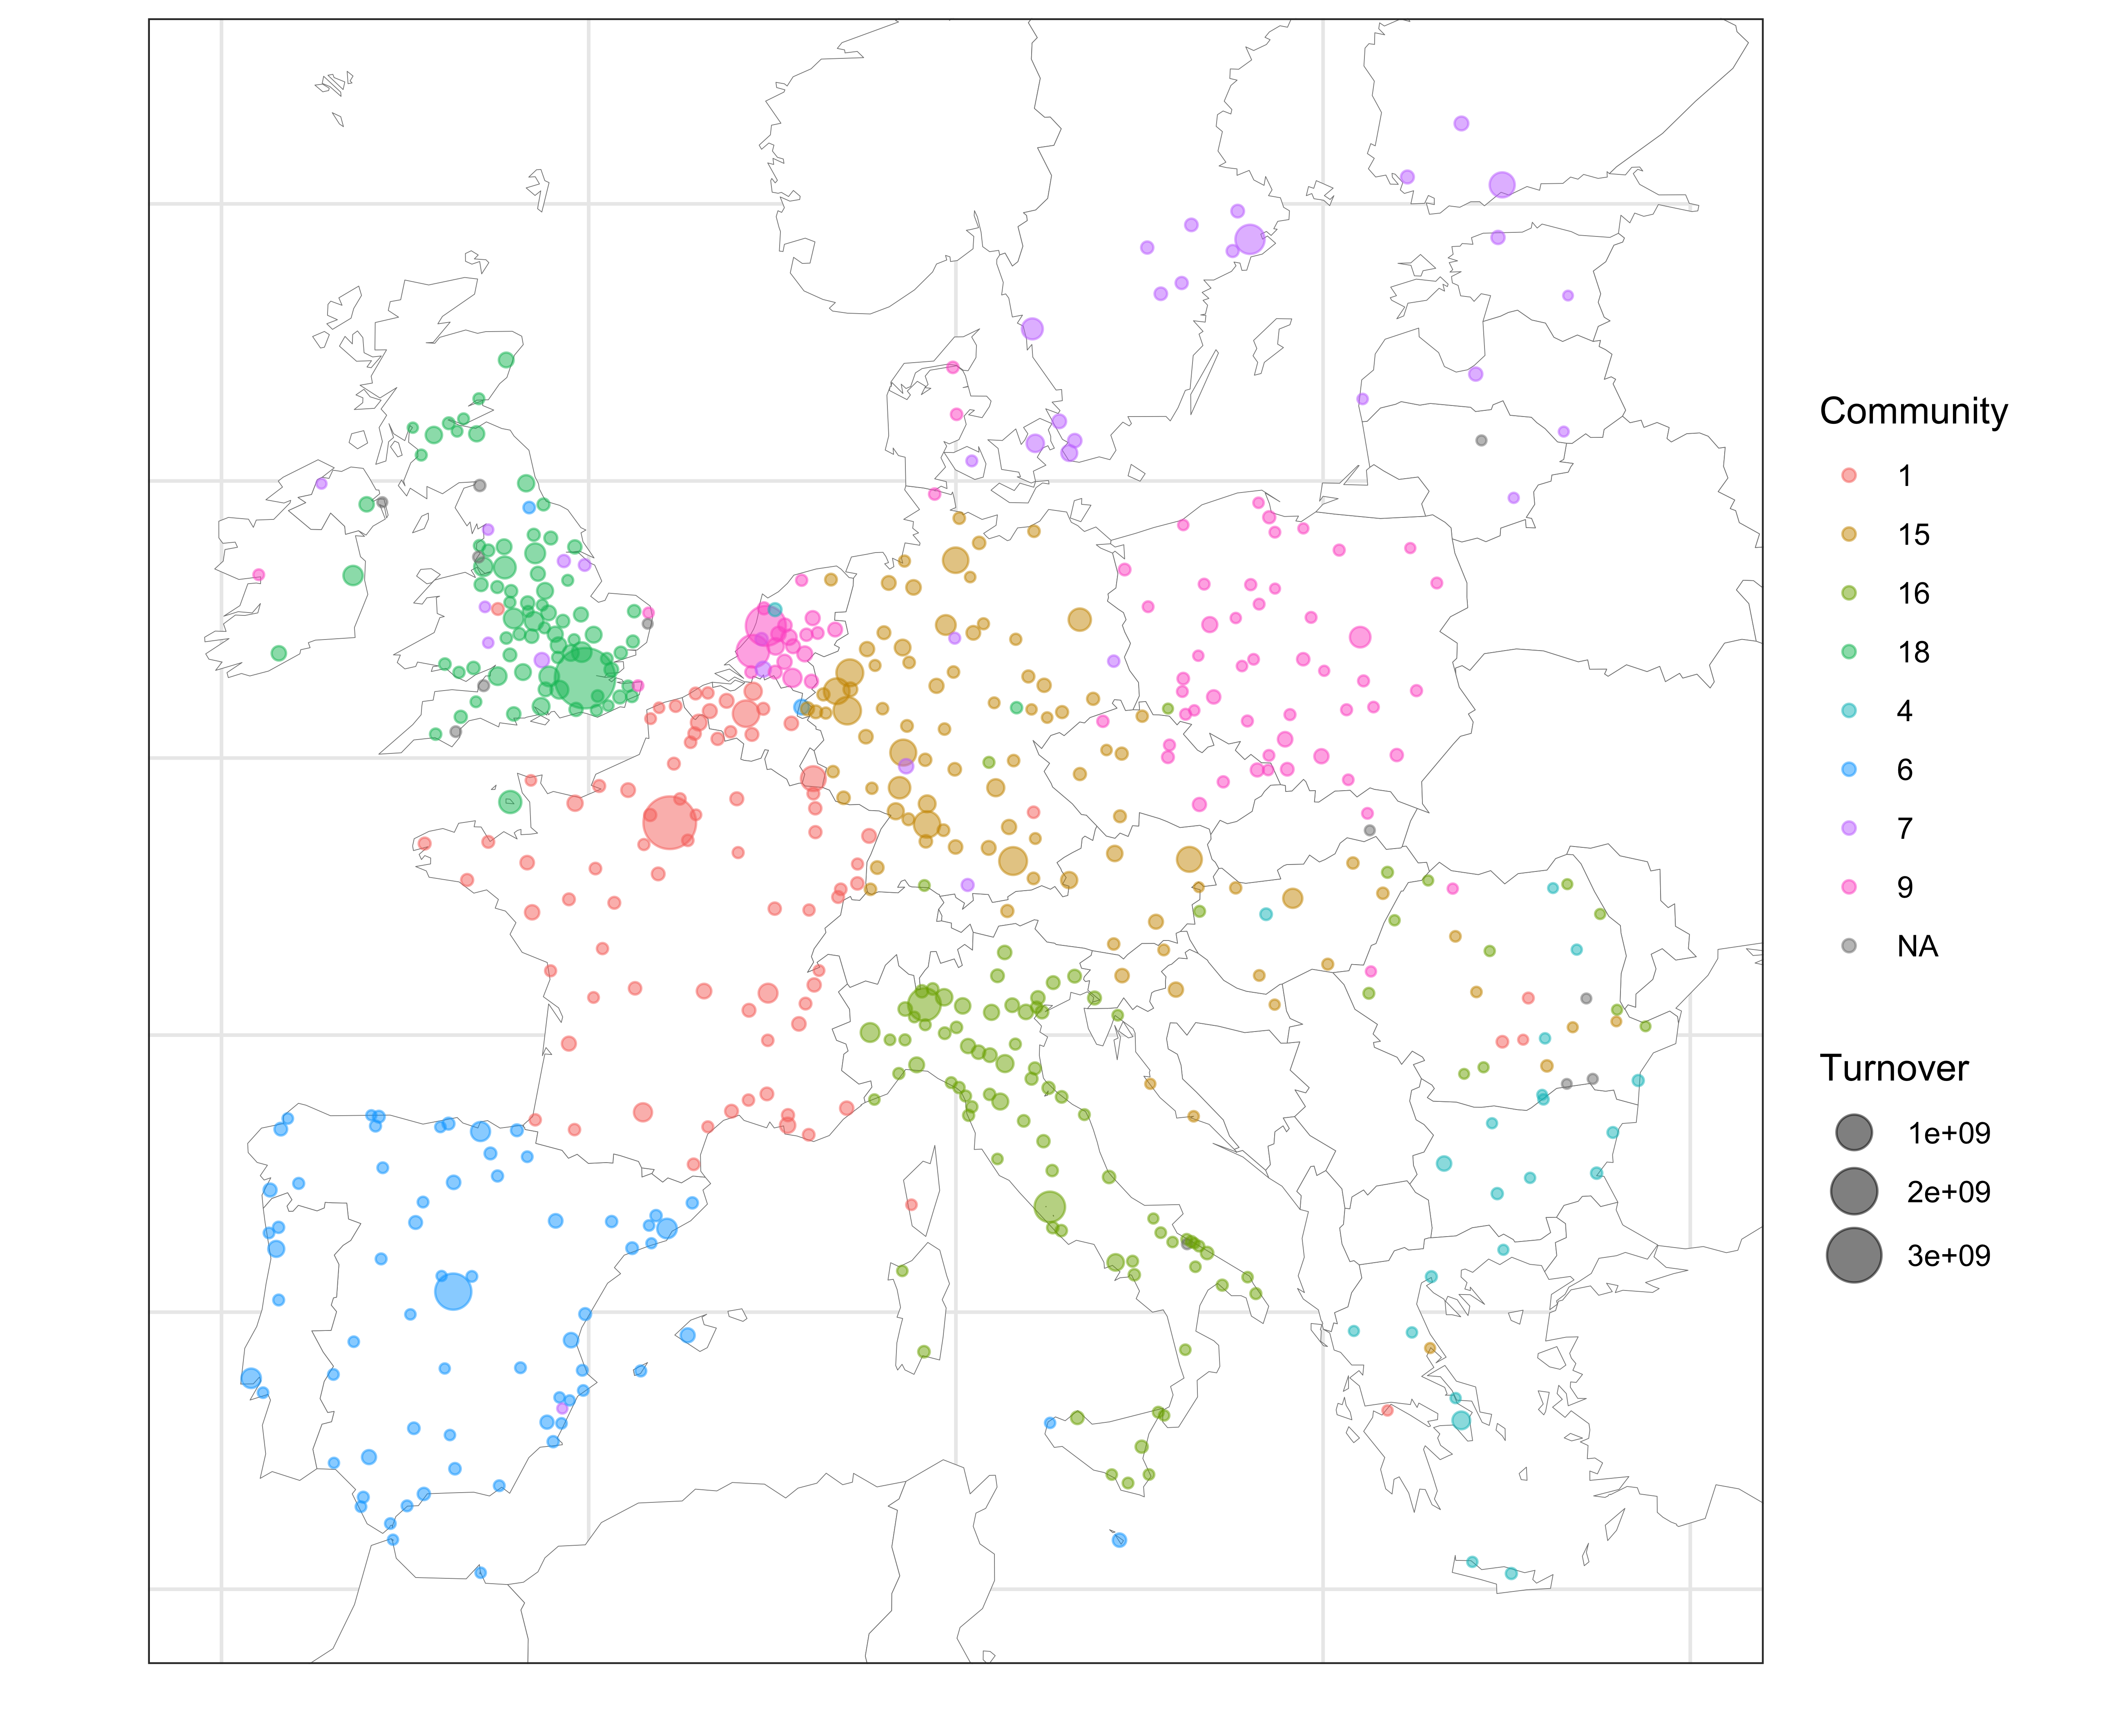
\includegraphics[width=0.45\linewidth]{../figures/Fig2.png}
    \includegraphics[width=0.42\linewidth]{../figures/Fig3.png}
    \caption{(Left) Empirical analysis of the AMADEUS data: urban area size corresponds to economic size, while color gives the community obtained with a Louvain modularity optimisation algorithm; (Right) Example of simulated networks: top row in a synthetic system with long-range interactions (left) and short range interactions (right), bottom row with same parameter values but in the real setting.}
\end{figure}

\end{document}
